\documentclass{article}

\usepackage[
    paperheight=10cm,
    paperwidth=10cm
  ]{geometry}

\usepackage{Archivo}
\usepackage[T1]{fontenc}

\usepackage{tikz}
\usepackage{xcolor}

\begin{document}
\nopagecolor 

\pagestyle{empty}

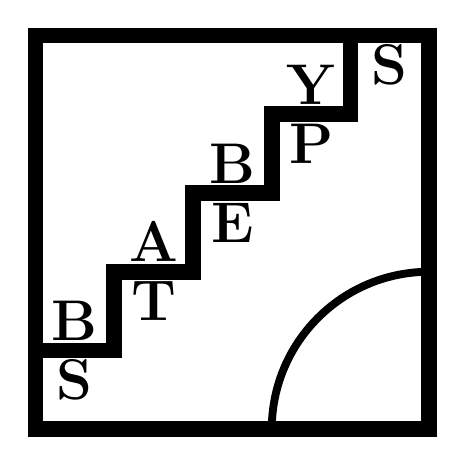
\begin{tikzpicture}
  \draw[line width=.2cm] (0,0) rectangle (5, 5);
  \draw[line width=.2cm] (0, 1) -- (1, 1) -- (1, 2) -- (2, 2) -- (2, 3) -- (3, 3) -- (3, 4) -- (4, 4) -- (4, 5);

  \node[anchor=south] at (.5, 1) {\bfseries\huge B};
  \node[anchor=south] at (1.5, 2) {\bfseries\huge A};
  \node[anchor=south] at (2.5, 3) {\bfseries\huge B};
  \node[anchor=south] at (3.5, 4) {\bfseries\huge Y};


  \node[anchor=north] at (.5, 1) {\bfseries\huge S};
  \node[anchor=north] at (1.5, 2) {\bfseries\huge T};
  \node[anchor=north] at (2.5, 3) {\bfseries\huge E};
  \node[anchor=north] at (3.5, 4) {\bfseries\huge P};
  \node[anchor=north] at (4.5, 5) {\bfseries\huge S};

  \draw[line width=.1cm] (3, 0) arc (180:90:2);

\end{tikzpicture}
\end{document}
